\chapter{\SwitchCaseDefaultSectionName}
\index{\CLanguageElements!switch}

% sections
\section{\RU{Если вариантов мало}\EN{Small number of cases}}

\lstinputlisting{patterns/08_switch/1_few/few.c}

\EN{\subsubsection{x86}

\myparagraph{\NonOptimizing MSVC}

Result (MSVC 2010):

\lstinputlisting[caption=MSVC 2010]{patterns/08_switch/1_few/few_msvc.asm}

Our function with a few cases in switch() is in fact analogous to this construction:

\lstinputlisting[label=switch_few_ifelse]{patterns/08_switch/1_few/few_analogue.c}

\myindex{\CLanguageElements!switch}
\myindex{\CLanguageElements!if}

If we work with switch() with a few cases it is impossible to be sure if it was
a real switch() in the source code, or just a pack of if() statements.
\myindex{\SyntacticSugar}

This implies that switch() is like syntactic sugar for a large number of nested if()s.

There is nothing especially new to us in the generated code,
with the exception of the compiler moving input variable $a$ to a temporary local variable \TT{tv64}
\footnote{Local variables in stack are prefixed with \TT{tv}---that's how MSVC names internal variables for its needs}.

If we compile this in GCC 4.4.1, we'll get almost the same result, even with maximal optimization
turned on (\Othree option).

\myparagraph{\Optimizing MSVC}

% TODO separate various kinds of \TT
% idea: enclose command lines in a specific environment, like \cmdline{} 
% assembly instructions in \asm{} (now both \TT and \q{} are used),
% variables in,  like \var{}
% messages (string constants) in something else, like \strconst
% to separate them all. Now they all use \TT, which is not best
% \INS{} for all instructions including operands? --DY
Now let's turn on optimization in MSVC (\Ox): \TT{cl 1.c /Fa1.asm /Ox}

\label{JMP_instead_of_RET}
\lstinputlisting[caption=MSVC]{patterns/08_switch/1_few/few_msvc_Ox.asm}

Here we can see some dirty hacks.

\myindex{x86!\Instructions!JZ}
\myindex{x86!\Instructions!JE}
\myindex{x86!\Instructions!SUB}

First: the value of $a$ is placed in \EAX and 0 is subtracted from it. Sounds absurd, but it is done to check if 
the value in \EAX was 0. If yes, the \ZF flag is to be set (e.g. subtracting from 0 is 0) 
and the first conditional jump \JE (\IT{Jump if Equal} or synonym \JZ~---\IT{Jump if Zero}) is to be triggered 
and control flow is to be passed to the \TT{\$LN4@f} label, where the \TT{'zero'} message is being printed. 
If the first jump doesn't get triggered, 1 is subtracted from the input value and if at some stage the result is 0, 
the corresponding jump is to be triggered.

And if no jump gets triggered at all, the control flow passes to \printf with string argument \\
\TT{'something unknown'}.

\label{jump_to_last_printf}
\myindex{\Stack}

Second: we see something unusual for us: a string pointer is placed into the $a$ variable, and 
then \printf is called not via \CALL, but via \JMP. There is a simple explanation for that: 
the \gls{caller} pushes a value to the stack and calls our function via \CALL. 
\CALL itself pushes the return address (\ac{RA}) to the stack and does an unconditional jump to our function address. 
Our function at any point of execution (since it do not contain any instruction that moves the stack 
pointer) has the following stack layout:

\begin{itemize}
\item\ESP---points to \ac{RA}
\item\TT{ESP+4}---points to the $a$ variable 
\end{itemize}

On the other side, when we need to call \printf here we need exactly the same stack 
layout, except for the first \printf argument, which needs to point to the string. 
And that is what our code does.

It replaces the function's first argument with the address of the string and 
jumps to \printf, as if we didn't call our function \ttf, but directly \printf.
\printf prints a string to \gls{stdout} and then executes the \RET instruction, which POPs 
\ac{RA} from the stack and control flow is returned not to \ttf but rather to \ttf's \gls{callee}, 
bypassing the end of the \ttf function.

\myindex{\CStandardLibrary!longjmp()}
\newcommand{\URLSJ}{\href{http://go.yurichev.com/17121}{wikipedia}}

All this is possible because \printf is called right at the end of the \ttf function in all cases. 
In some way, it is similar to the \TT{longjmp()}\footnote{\URLSJ} function.
And of course, it is all done for the sake of speed.

A similar case with the ARM compiler is described in \q{\PrintfSeveralArgumentsSectionName}
section, here~(\myref{ARM_B_to_printf}).

\clearpage
\myparagraph{\olly}

Since this example is tricky, let's trace it in \olly.

\olly can detect such switch() constructs, and it can add some useful comments.
\EAX is 2 in the beginning, that's the function's input value: 

\begin{figure}[H]
\centering
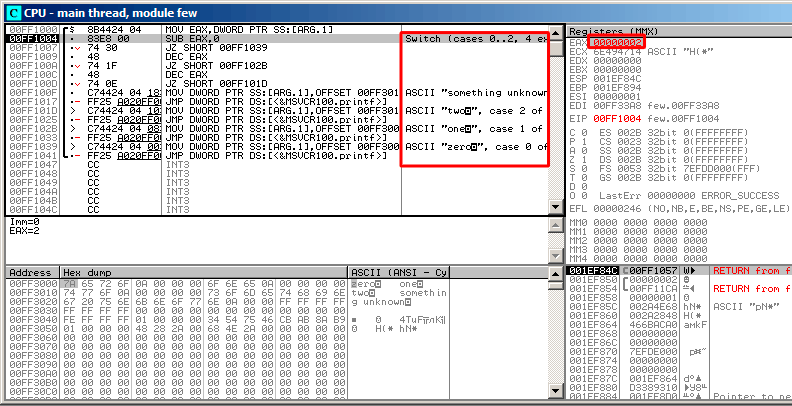
\includegraphics[scale=\FigScale]{patterns/08_switch/1_few/olly1.png}
\caption{\olly: \EAX 
now contain the first (and only) function argument}
\label{fig:switch_few_olly1}
\end{figure}

\clearpage
0 is subtracted from 2 in \EAX. 
Of course, \EAX still contains 2.
But the \ZF flag is now 0, indicating that the resulting value is non-zero:

\begin{figure}[H]
\centering
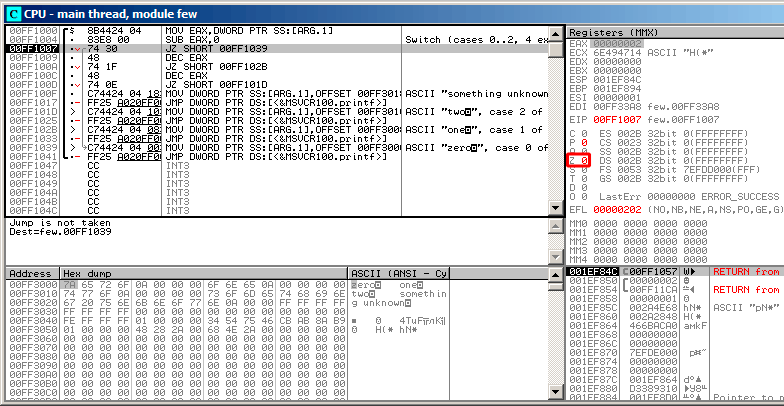
\includegraphics[scale=\FigScale]{patterns/08_switch/1_few/olly2.png}
\caption{\olly: \SUB executed}
\label{fig:switch_few_olly2}
\end{figure}

\clearpage
\DEC is executed and \EAX now contains 1. 
But 1 is non-zero, so the \ZF flag is still 0:

\begin{figure}[H]
\centering
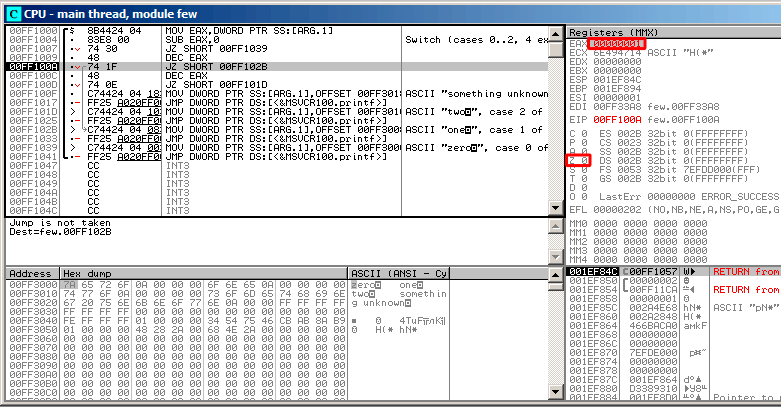
\includegraphics[scale=\FigScale]{patterns/08_switch/1_few/olly3.png}
\caption{\olly: first \DEC executed}
\label{fig:switch_few_olly3}
\end{figure}

\clearpage
Next \DEC is executed. 
\EAX is finally 0 and the \ZF flag gets set, because the result is zero:

\begin{figure}[H]
\centering
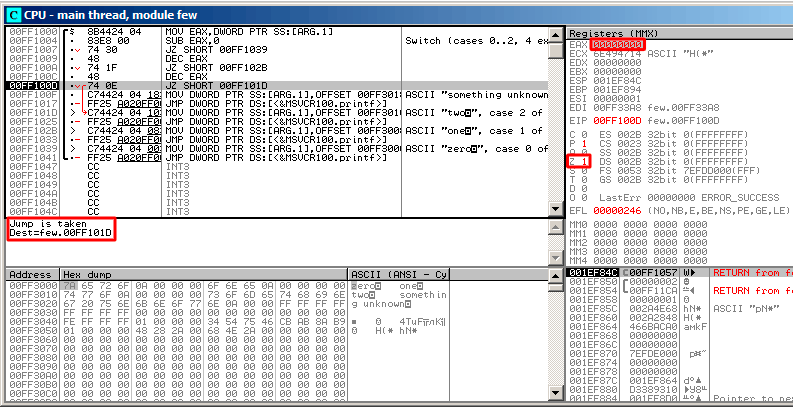
\includegraphics[scale=\FigScale]{patterns/08_switch/1_few/olly4.png}
\caption{\olly: second \DEC executed}
\label{fig:switch_few_olly4}
\end{figure}

\olly shows that this jump is to be taken now.

\clearpage
A pointer to the string \q{two} is to be written into the stack now:

\begin{figure}[H]
\centering
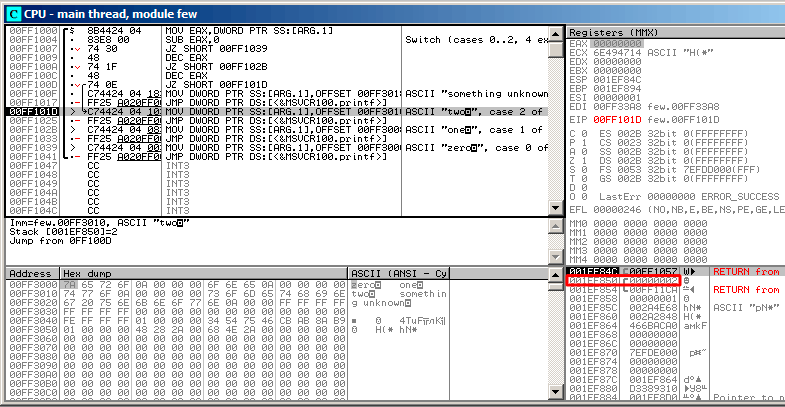
\includegraphics[scale=\FigScale]{patterns/08_switch/1_few/olly5.png}
\caption{\olly: 
pointer to the string is to be written at the place of the first argument}
\label{fig:switch_few_olly5}
\end{figure}

% TODO: homogenize numbers
% now they are inconsistent: sometimes plain text, sometimes in math mode
% some kind of \expr{} both for numbers and expressions? --DY
Please note: the current argument of the function is 2 and 2 is now in the stack at the address \TT{0x001EF850}.

\clearpage
\MOV writes the pointer to the string at address \TT{0x001EF850} (see the stack window).
Then, jump happens.
This is the first instruction of the \printf function in MSVCR100.DLL (This example was compiled with /MD switch): 

\begin{figure}[H]
\centering
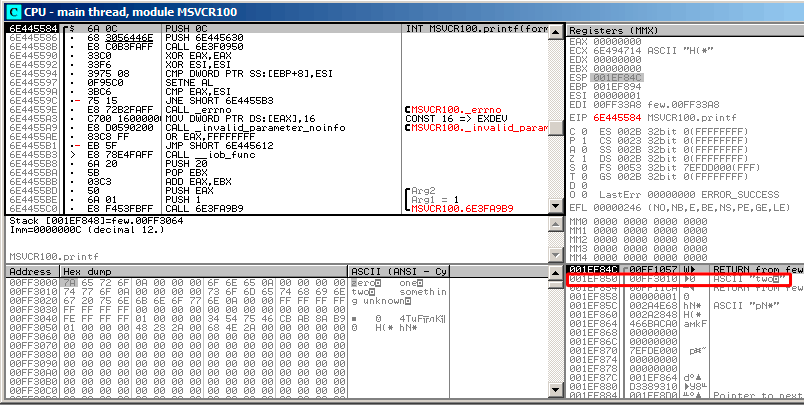
\includegraphics[scale=\FigScale]{patterns/08_switch/1_few/olly6.png}
\caption{\olly: first instruction of \printf \InENRU MSVCR100.DLL}
\label{fig:switch_few_olly6}
\end{figure}

Now \printf treats the string at \TT{0x00FF3010} as its only argument and prints the string.

\clearpage
This is the last instruction of \printf:

\begin{figure}[H]
\centering
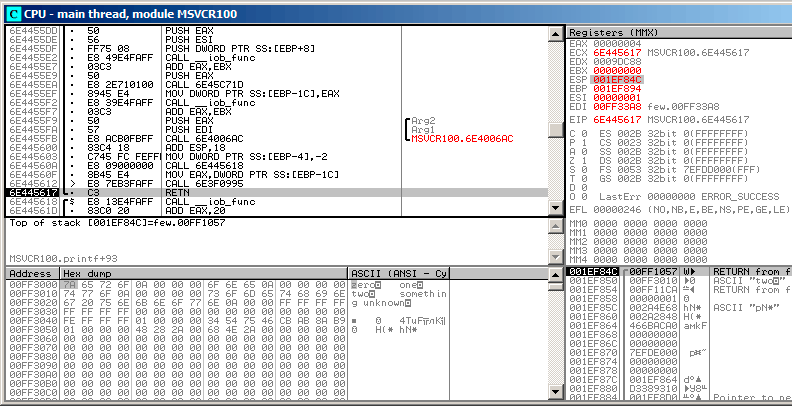
\includegraphics[scale=\FigScale]{patterns/08_switch/1_few/olly7.png}
\caption{\olly: last instruction of \printf in MSVCR100.DLL}
\label{fig:switch_few_olly7}
\end{figure}

The string \q{two} was just printed to the console window.

\clearpage
Now let's press F7 or F8 (\stepover) and return\dots not to \ttf , but rather to \main:

\begin{figure}[H]
\centering
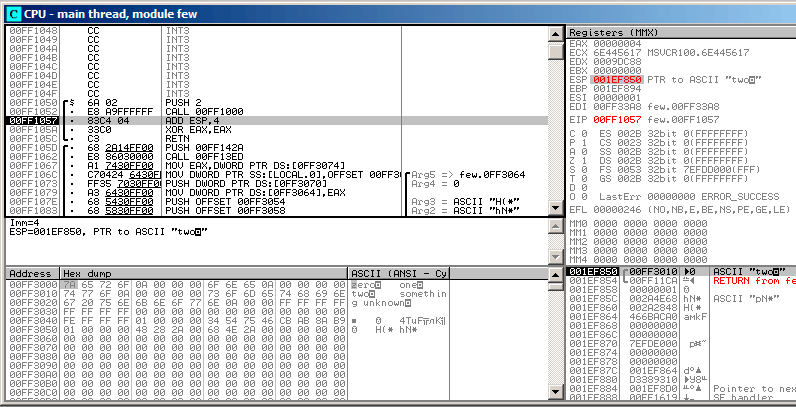
\includegraphics[scale=\FigScale]{patterns/08_switch/1_few/olly8.png}
\caption{\olly: return to \main}
\label{fig:switch_few_olly8}
\end{figure}

Yes, the jump was direct, from the guts of \printf to \main.
Because \ac{RA} in the stack points not to some place in \ttf , but rather to \main.
And \CALL \TT{0x00FF1000} was the actual instruction which called \ttf.



}
\RU{\subsubsection{x86}

\myparagraph{\NonOptimizing MSVC}

Это дает в итоге (MSVC 2010):

\lstinputlisting[caption=MSVC 2010]{patterns/08_switch/1_few/few_msvc.asm}

Наша функция со оператором switch(), с небольшим количеством вариантов, 
это практически аналог подобной конструкции:

\lstinputlisting[label=switch_few_ifelse]{patterns/08_switch/1_few/few_analogue.c}

\myindex{\CLanguageElements!switch}
\myindex{\CLanguageElements!if}
Когда вариантов немного и мы видим подобный код, невозможно сказать с уверенностью, был ли
в оригинальном исходном коде switch(), либо просто набор операторов if().

\myindex{\SyntacticSugar}
То есть, switch() это синтаксический сахар для большого количества вложенных проверок 
при помощи if().

В самом выходном коде ничего особо нового, 
за исключением того, что компилятор зачем-то 
перекладывает входящую переменную ($a$) во временную в локальном стеке \TT{v64}\footnote{Локальные переменные в стеке с префиксом \TT{tv}~--- 
так MSVC называет внутренние переменные для своих нужд}.

Если скомпилировать это при помощи GCC 4.4.1, то будет почти то же самое, даже с максимальной оптимизацией (ключ \Othree).

\myparagraph{\Optimizing MSVC}

% TODO separate various kinds of \TT
% idea: enclose command lines in a specific environment, like \cmdline{} 
% assembly instructions in \asm{} (now both \TT and \q{} are used),
% variables in,  like \var{}
% messages (string constants) in something else, like \strconst
% to separate them all. Now they all use \TT, which is not best
% \INS{} for all instructions including operands? --DY

Попробуем включить оптимизацию кодегенератора MSVC (\Ox): \TT{cl 1.c /Fa1.asm /Ox}

\label{JMP_instead_of_RET}
\lstinputlisting[caption=MSVC]{patterns/08_switch/1_few/few_msvc_Ox.asm}

Вот здесь уже всё немного по-другому, причем не без грязных трюков.

\myindex{x86!\Instructions!JZ}
\myindex{x86!\Instructions!JE}
\myindex{x86!\Instructions!SUB}
Первое: \TT{а} помещается в \EAX и от него отнимается 0. Звучит абсурдно, но нужно это для того, чтобы проверить, 
0 ли в \EAX был до этого? Если да, то выставится флаг \ZF (что означает, что результат вычитания 0 от числа 
стал 0) и первый условный переход \JE (\IT{Jump if Equal} или его синоним \JZ~--- \IT{Jump if Zero}) 
сработает на метку \TT{\$LN4@f}, где выводится сообщение \TT{'zero'}.
Если первый переход не сработал, от значения отнимается по единице, 
и если на какой-то стадии в результате образуется 0, то сработает соответствующий переход.

И в конце концов, если ни один из условных переходов не сработал, управление передается \printf
со строковым аргументом \TT{'something unknown'}.

\label{jump_to_last_printf}
\myindex{\Stack}
Второе: мы видим две, мягко говоря, необычные вещи: указатель на сообщение помещается в переменную $a$, 
и затем \printf вызывается не через \CALL, а через \JMP. Объяснение этому простое. 
Вызывающая функция заталкивает в стек некоторое значение и через \CALL вызывает нашу функцию. 
\CALL в свою очередь заталкивает в стек адрес возврата (\ac{RA}) и делает безусловный переход на адрес нашей функции. 
Наша функция в самом начале (да и в любом её месте, потому что в теле функции нет ни одной инструкции, 
которая меняет что-то в стеке или в \ESP) имеет следующую разметку стека:

\begin{itemize}
\item\ESP --- хранится \ac{RA}
\item\TT{ESP+4} --- хранится значение $a$ 
\end{itemize}

С другой стороны, чтобы вызвать \printf, нам нужна почти такая же разметка стека, 
только в первом аргументе нужен указатель на строку. Что, собственно, этот код и делает.

Он заменяет свой первый аргумент на адрес строки, и затем передает управление \printf, как если бы вызвали не 
нашу функцию \ttf, а сразу \printf. 
\printf выводит некую строку на \gls{stdout}, затем исполняет инструкцию \RET, 
которая из стека достает \ac{RA} и управление передается в ту функцию, 
которая вызывала \ttf, минуя при этом конец функции \ttf.

\myindex{\CStandardLibrary!longjmp()}
\newcommand{\URLSJ}{\href{http://go.yurichev.com/17121}{wikipedia}}
Всё это возможно, потому что \printf вызывается в \ttf в самом конце. 
Всё это чем-то даже похоже на \TT{longjmp()}\footnote{\URLSJ}.
И всё это, разумеется, сделано для экономии времени исполнения.

Похожая ситуация с компилятором для ARM описана в секции \q{\PrintfSeveralArgumentsSectionName}~(\myref{ARM_B_to_printf}).

\clearpage
\myparagraphold{\olly}

Так как этот пример немного запутанный, попробуем оттрассировать его в \olly.

\olly может распознавать подобные switch()-конструкции, так что он добавляет полезные комментарии.
\EAX в начале равен 2, это входное значение функции: 

\begin{figure}[H]
\centering
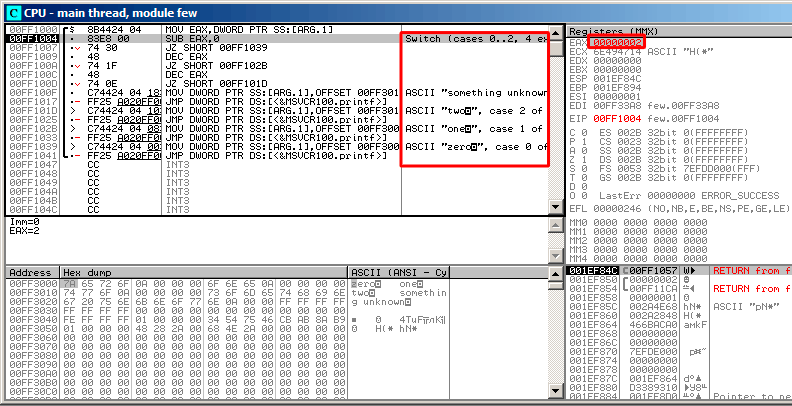
\includegraphics[scale=\FigScale]{patterns/08_switch/1_few/olly1.png}
\caption{\olly: \EAX содержит первый (и единственный) аргумент функции}
\label{fig:switch_few_olly1}
\end{figure}

\clearpage
0 отнимается от 2 в \EAX. 
Конечно же, \EAX всё ещё содержит 2.
Но флаг \ZF теперь 0, что означает, что последнее вычисленное значение не было нулевым:

\begin{figure}[H]
\centering
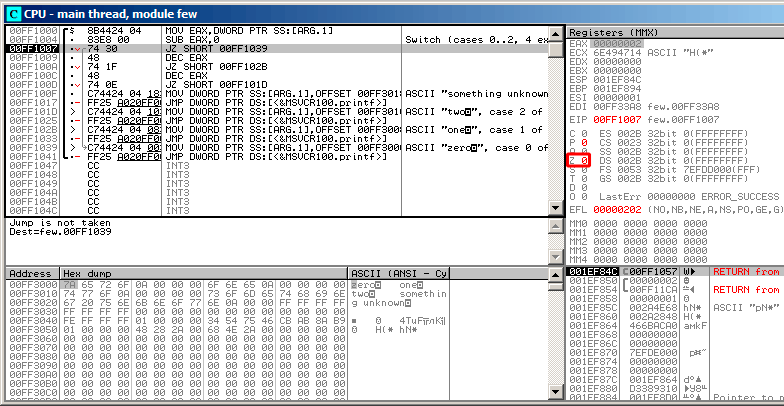
\includegraphics[scale=\FigScale]{patterns/08_switch/1_few/olly2.png}
\caption{\olly: \SUB исполнилась}
\label{fig:switch_few_olly2}
\end{figure}

\clearpage
\DEC исполнилась и \EAX теперь содержит 1. 
Но 1 не ноль, так что флаг \ZF всё ещё 0:

\begin{figure}[H]
\centering
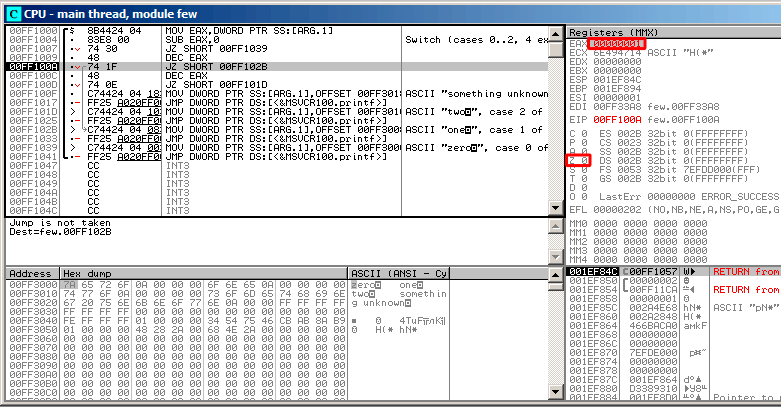
\includegraphics[scale=\FigScale]{patterns/08_switch/1_few/olly3.png}
\caption{\olly: первая \DEC исполнилась}
\label{fig:switch_few_olly3}
\end{figure}

\clearpage
Следующая \DEC исполнилась. 
\EAX наконец 0 и флаг \ZF выставлен, потому что результат~--- ноль:

\begin{figure}[H]
\centering
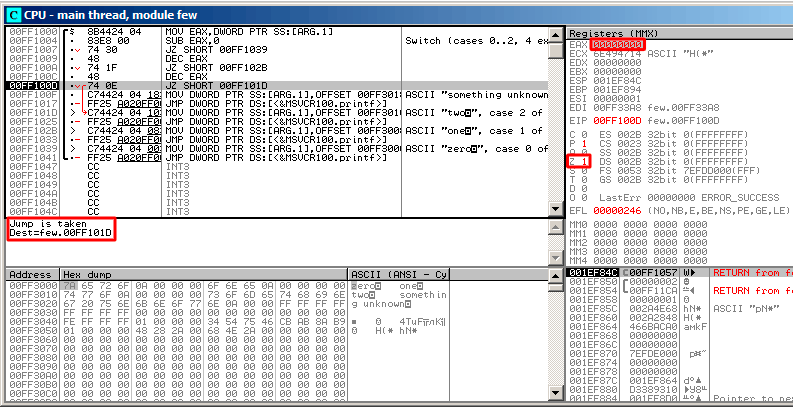
\includegraphics[scale=\FigScale]{patterns/08_switch/1_few/olly4.png}
\caption{\olly: вторая \DEC исполнилась}
\label{fig:switch_few_olly4}
\end{figure}

\olly показывает, что условный переход сейчас сработает.

\clearpage
Указатель на строку \q{two} 
сейчас будет записан в стек:

\begin{figure}[H]
\centering
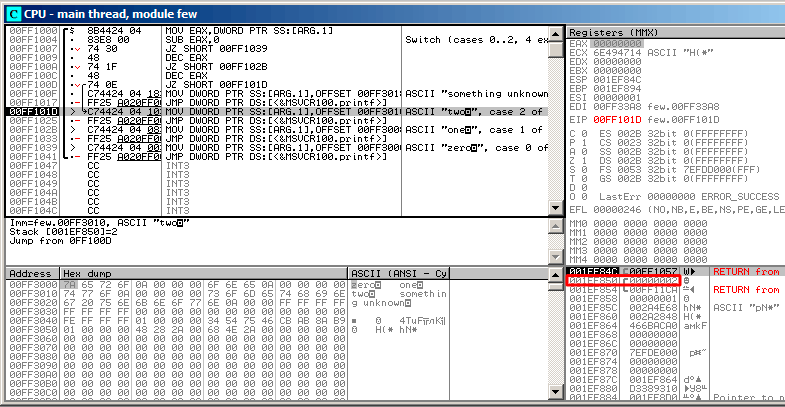
\includegraphics[scale=\FigScale]{patterns/08_switch/1_few/olly5.png}
\caption{\olly: указатель на строку сейчас запишется на место первого аргумента}
\label{fig:switch_few_olly5}
\end{figure}

% TODO: homogenize numbers
% now they are inconsistent: sometimes plain text, sometimes in math mode
% some kind of \expr{} both for numbers and expressions? --DY
Обратите внимание: текущий аргумент функции это 2 и 2 прямо сейчас в стеке по адресу \TT{0x001EF850}.

\clearpage
\MOV записывает указатель на строку по адресу \TT{0x001EF850} (см. окно стека).
Переход сработал.
Это самая первая инструкция функции \printf в MSVCR100.DLL (этот пример был скомпилирован с опцией /MD): 

\begin{figure}[H]
\centering
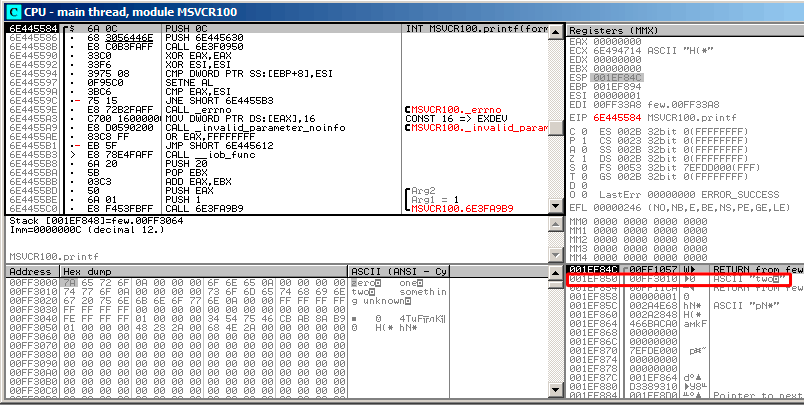
\includegraphics[scale=\FigScale]{patterns/08_switch/1_few/olly6.png}
\caption{\olly: первая инструкция в \printf в MSVCR100.DLL}
\label{fig:switch_few_olly6}
\end{figure}

Теперь \printf считает строку на \TT{0x00FF3010} как свой единственный аргумент и выводит строку.

\clearpage
Это самая последняя инструкция функции \printf:

\begin{figure}[H]
\centering
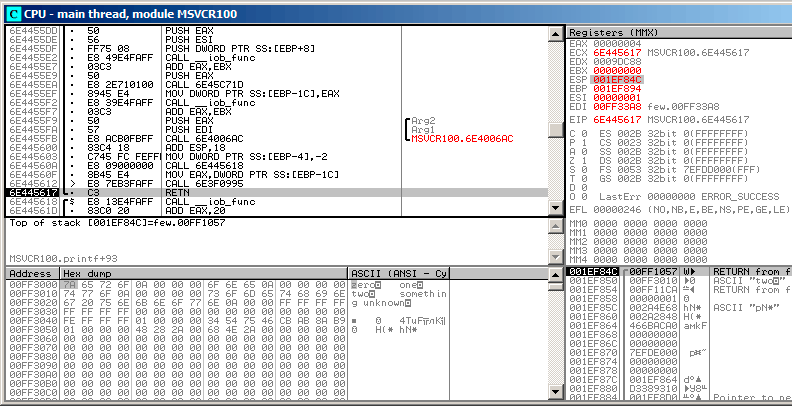
\includegraphics[scale=\FigScale]{patterns/08_switch/1_few/olly7.png}
\caption{\olly: последняя инструкция в \printf в MSVCR100.DLL}
\label{fig:switch_few_olly7}
\end{figure}

Строка \q{two} была только что выведена в консоли.

\clearpage
Нажмем F7 или F8 (\stepover) и вернемся\dots нет, не в функцию \ttf но в \main:

\begin{figure}[H]
\centering
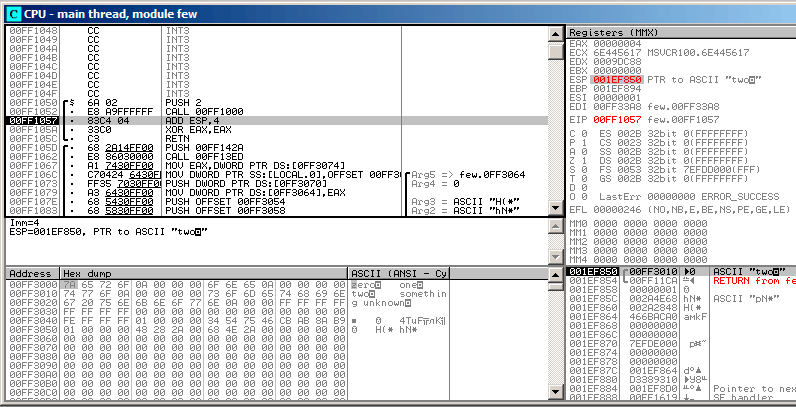
\includegraphics[scale=\FigScale]{patterns/08_switch/1_few/olly8.png}
\caption{\olly: возврат в \main}
\label{fig:switch_few_olly8}
\end{figure}

Да, это прямой переход из внутренностей \printf в \main.
Потому как \ac{RA} в стеке указывает не на какое-то место в функции \ttf а в \main.
И \CALL \TT{0x00FF1000} это инструкция вызывающая функцию \ttf.



}
\EN{\subsubsection{ARM: \OptimizingKeilVI (\ARMMode)}
\myindex{\CLanguageElements!switch}

\lstinputlisting{patterns/08_switch/1_few/few_ARM_ARM_O3.asm}

Again, by investigating this code we cannot say if it was a switch() in the original source code, 
or just a pack of if() statements.

\myindex{ARM!\Instructions!ADRcc}

Anyway, we see here predicated instructions again (like \ADREQ (\IT{Equal}))
which is triggered only in case $R0=0$, and then loads the address of the string \IT{<<zero\textbackslash{}n>>}
into \Reg{0}.
\myindex{ARM!\Instructions!BEQ}
The next instruction \ac{BEQ} redirects control flow to \TT{loc\_170}, if $R0=0$.

An astute reader may ask, will \ac{BEQ} trigger correctly since \ADREQ it
has already filled the \Reg{0} register before with another value?

Yes, it will since \ac{BEQ} checks the flags set by the \CMP instruction, 
and \ADREQ does not modify any flags at all.

The rest of the instructions are already familiar to us. 
There is only one call to \printf , at the end, and we have already examined this trick here~(\myref{ARM_B_to_printf}).
At the end, there are three paths to \printf{}.

\myindex{ARM!\Instructions!ADRcc}
\myindex{ARM!\Instructions!CMP}
The last instruction, \TT{CMP R0, \#2}, is needed to check if $a=2$.

If it is not true, then \ADRNE loads a pointer to the string \IT{<<something unknown \textbackslash{}n>>}
into \Reg{0}, since $a$ has already been checked to be equal to 0 or 1,
and we can sure that the $a$ variable is not equal to these numbers at this point.
And if $R0=2$, 
a pointer to the string \IT{<<two\textbackslash{}n>>}
will be loaded by \ADREQ into \Reg{0}.

\subsubsection{ARM: \OptimizingKeilVI (\ThumbMode)}

\lstinputlisting{patterns/08_switch/1_few/few_ARM_thumb_O3.asm}

% FIXME а каким можно? к каким нельзя? \myref{} ->

As was already mentioned, it is not possible to add conditional predicates to most instructions in Thumb
mode, so the Thumb-code here is somewhat similar to the easily understandable x86 \ac{CISC}-style code.

\subsubsection{ARM64: \NonOptimizing GCC (Linaro) 4.9}

\lstinputlisting{patterns/08_switch/1_few/ARM64_GCC_O0_EN.lst}

The type of the input value is \Tint, hence register \RegW{0} is used to hold it instead of the whole
\RegX{0} register.

The string pointers are passed to \puts using an \INS{ADRP}/\INS{ADD} instructions pair just like it was demonstrated in the 
\q{\HelloWorldSectionName} example:~\myref{pointers_ADRP_and_ADD}.

\subsubsection{ARM64: \Optimizing GCC (Linaro) 4.9}

\lstinputlisting{patterns/08_switch/1_few/ARM64_GCC_O3_EN.lst}

Better optimized piece of code.
\TT{CBZ} (\IT{Compare and Branch on Zero}) instruction does jump if \RegW{0} is zero.
There is also a direct jump to \puts instead of calling it, like it was explained before:~\myref{JMP_instead_of_RET}.

}
\RU{\subsectionold{ARM: \OptimizingKeilVI (\ARMMode)}
\myindex{\CLanguageElements!switch}

\lstinputlisting{patterns/08_switch/1_few/few_ARM_ARM_O3.asm}

Мы снова не сможем сказать, глядя на этот код, был ли в оригинальном исходном коде switch() 
либо же несколько операторов if().

\myindex{ARM!\Instructions!ADRcc}
Так или иначе, мы снова видим здесь инструкции с предикатами, например, \ADREQ (\IT{(Equal)}), 
которая будет исполняться только
если $R0=0$, и тогда в \Reg{0} будет загружен адрес строки \IT{<<zero\textbackslash{}n>>}.

\myindex{ARM!\Instructions!BEQ}
Следующая инструкция \ac{BEQ} перенаправит исполнение на \TT{loc\_170}, если $R0=0$.

Кстати, наблюдательный читатель может спросить, сработает ли \ac{BEQ} нормально,
ведь \ADREQ перед ним уже заполнила регистр \Reg{0} чем-то другим?

Сработает, потому что \ac{BEQ} проверяет флаги, установленные инструкцией \CMP, 
а \ADREQ флаги никак не модифицирует.

Далее всё просто и знакомо. 
Вызов \printf один, и в самом конце, мы уже рассматривали подобный трюк~(\myref{ARM_B_to_printf}).
К вызову функции \printf{} в конце ведут три пути.

\myindex{ARM!\Instructions!ADRcc}
\myindex{ARM!\Instructions!CMP}
Последняя инструкция \TT{CMP R0, \#2} здесь нужна, чтобы узнать $a=2$ или нет.

Если это не так, то при помощи \ADRNE (\IT{Not Equal}) в \Reg{0} будет загружен указатель на 
строку \IT{<<something unknown \textbackslash{}n>>}, ведь $a$ уже было проверено на 0 и 1 до этого, 
и здесь $a$ точно не попадает под эти константы.

Ну а если $R0=2$, в \Reg{0} будет загружен указатель на строку \IT{<<two\textbackslash{}n>>} при помощи инструкции \ADREQ.

\subsectionold{ARM: \OptimizingKeilVI (\ThumbMode)}

\lstinputlisting{patterns/08_switch/1_few/few_ARM_thumb_O3.asm}

% FIXME а каким можно? к каким нельзя? \myref{} ->
Как уже было отмечено, в Thumb-режиме нет возможности добавлять условные предикаты к большинству инструкций,
так что Thumb-код вышел похожим на код x86 в стиле \ac{CISC}, вполне понятный.

\subsectionold{ARM64: \NonOptimizing GCC (Linaro) 4.9}

\lstinputlisting{patterns/08_switch/1_few/ARM64_GCC_O0_RU.lst}

Входное значение имеет тип \Tint, поэтому для него используется регистр \RegW{0},
а не целая часть регистра \RegX{0}.

Указатели на строки передаются в \puts при помощи пары инструкций ADRP/ADD, как было показано в примере
\q{\HelloWorldSectionName}:~\myref{pointers_ADRP_and_ADD}.

\subsectionold{ARM64: \Optimizing GCC (Linaro) 4.9}

\lstinputlisting{patterns/08_switch/1_few/ARM64_GCC_O3_RU.lst}

Фрагмент кода более оптимизированный.
Инструкция \TT{CBZ} (\IT{Compare and Branch on Zero}~--- сравнить и перейти если ноль) совершает переход если \RegW{0} ноль.
Здесь также прямой переход на \puts вместо вызова, как уже было описано:~\myref{JMP_instead_of_RET}.

}
\EN{\subsubsection{MIPS}

\lstinputlisting[caption=\Optimizing GCC 4.4.5 (IDA)]{patterns/08_switch/1_few/MIPS_O3_IDA_EN.lst}

\myindex{MIPS!\Instructions!JR}

The function always ends with calling \puts, so here we see a jump to \puts (\INS{JR}: \q{Jump Register}) instead of \q{jump and link}.
We talked about this earlier: \myref{JMP_instead_of_RET}.

\myindex{MIPS!Load delay slot}
We also often see \INS{NOP} instructions after \INS{LW} ones.
This is \q{load delay slot}: another \IT{delay slot} in MIPS.
\myindex{MIPS!\Instructions!LW}

An instruction next to \INS{LW} may execute at the moment while \INS{LW} loads value from memory. 

However, the next instruction must not use the result of \INS{LW}.

Modern MIPS CPUs have a feature to wait if the next instruction uses result of \INS{LW}, so this is somewhat outdated,
but GCC still adds NOPs for older MIPS CPUs.
In general, it can be ignored.
}
\RU{\subsubsection{MIPS}

\lstinputlisting[caption=\Optimizing GCC 4.4.5 (IDA)]{patterns/08_switch/1_few/MIPS_O3_IDA_RU.lst}

\myindex{MIPS!\Instructions!JR}

Функция всегда заканчивается вызовом \puts, так что здесь мы видим переход на \puts (\INS{JR}: \q{Jump Register})
вместо перехода с сохранением \ac{RA} (\q{jump and link}).

Мы говорили об этом ранее: \myref{JMP_instead_of_RET}.

\myindex{MIPS!Load delay slot}
Мы также часто видим NOP-инструкции после \INS{LW}.
Это \q{load delay slot}: ещё один \IT{delay slot} в MIPS.
\myindex{MIPS!\Instructions!LW}
Инструкция после \INS{LW} может исполняться в тот момент, когда \INS{LW} загружает значение из памяти.

Впрочем, следующая инструкция не должна использовать результат \INS{LW}.

Современные MIPS-процессоры ждут, если следующая инструкция использует результат \INS{LW}, так что всё это уже
устарело, но GCC всё еще добавляет NOP-ы для более старых процессоров.

Вообще, это можно игнорировать.

}

\subsection{\Conclusion{}}

\EN{A \IT{switch()} with few cases is indistinguishable from an \IT{if/else} construction, for example:}
\RU{Оператор \IT{switch()} с малым количеством вариантов трудно отличим от применения конструкции \IT{if/else}:}
\lstref{switch_few_ifelse}.


\section{\RU{И если много}\EN{A lot of cases}}

\RU{А если ветвлений слишком много, то конечно генерировать слишком длинный код с многочисленными \JE/\JNE 
уже не так удобно.}
\EN{If a \TT{switch()} statement contains a lot of cases, it is not very convenient for the compiler to emit too large code
with a lot \JE/\JNE instructions.}

\lstinputlisting[label=switch_lot_c]{patterns/08_switch/2_lot/lot.c}

\subsection{x86}

\subsubsection{\NonOptimizing MSVC}

\RU{Имеем в итоге}\EN{We got} (MSVC 2010):

\lstinputlisting[caption=MSVC 2010]{patterns/08_switch/2_lot/lot_msvc.asm}

\index{jumptable}
\RU{Здесь происходит следующее: в теле функции есть набор вызовов \printf с разными аргументами. 
Все они имеют, конечно же, адреса, а также внутренние символические метки, которые присвоил им компилятор.
Также, все эти метки указываются во внутренней таблице \TT{\$LN11@f}.}
\EN{OK, what we see here is: there is a set of the \printf calls with various arguments. 
All they has not only addresses in process memory, but also internal symbolic labels assigned 
by compiler. 
All these labels are also mentioned in \TT{\$LN11@f} internal table.}

\RU{В начале функции, если $a$ больше 4, то сразу происходит переход на метку \TT{\$LN1@f}, 
где вызывается \printf с аргументом \TT{'something unknown'}.}
\EN{At the function beginning, if $a$ is greater than 4, control flow is passed to label 
\TT{\$LN1@f}, where \printf with argument \TT{'something unknown'} is called.}

\RU{А если $a$ меньше или равно 4, то это значение умножается на 4 и прибавляется адрес таблицы 
с переходами (\TT{\$LN11@f}). 
Таким образом, получается адрес внутри таблицы, где лежит нужный адрес внутри тела функции. 
Например, возьмем $a$ равным 2. $2*4 = 8$ (ведь все элементы таблицы ~--- это адреса внутри 32-битного процесса, 
таким образом, каждый элемент занимает 4 байта). 8 прибавить к \TT{\$LN11@f} ~--- это будет элемент таблицы,
где лежит \TT{\$LN4@f}. \JMP вытаскивает из таблицы адрес \TT{\$LN4@f} и делает безусловный переход туда.}
\EN{But if $a$ value is less or equals to 4, let's multiply it by 4 and add \TT{\$LN11@f} 
table address. That is how address inside of table is constructed, pointing exactly to the 
element we need. For example, let's say $a$ is equal to 2. $2*4 = 8$ (all table elements 
are addresses within 32-bit process that is why all elements contain 4 bytes). 
Address of the \TT{\$LN11@f} table + 8~---it will be table element where \TT{\$LN4@f} label is stored.
\JMP fetches \TT{\$LN4@f} address from the table and jump to it.}

\RU{Эта таблица иногда называется}\EN{This table sometimes called} \IT{jumptable} \OrENRU 
\IT{branch table}\footnote{\EN{The whole method once called}\RU{Сам метод раньше назывался} 
\IT{computed GOTO} \EN{in early FORTRAN versions}\RU{В ранних версиях FORTRAN}:
\url{http://en.wikipedia.org/wiki/Branch_table}.
\EN{Not quite relevant these days, but what a term}\RU{Не очень-то и полезно в наше время, но
каков термин}!}.

\RU{А там вызывается \printf с аргументом \TT{'two'}. 
Дословно, инструкция \TT{jmp DWORD PTR \$LN11@f[ecx*4]} 
означает \IT{перейти по DWORD, который лежит по адресу} \TT{\$LN11@f + ecx * 4}.}
\EN{Then corresponding \printf is called with argument \TT{'two'}. 
Literally, \TT{jmp DWORD PTR \$LN11@f[ecx*4]} instruction means
\IT{jump to DWORD, which is stored at address} \TT{\$LN11@f + ecx * 4}.}

\TT{npad}~(\ref{sec:npad})
\RU{это макрос ассемблера, немного выровнять начало таблицы, 
дабы она располагалась по 
адресу кратному 4 (или 16). Это нужно для того чтобы процессор мог эффективнее загружать 32-битное 
значения из памяти, через шину с памятью, кэш-память, и т.д.}
\EN{is assembly language macro, aligning next label so that it will be stored at address aligned on a 4 byte
(or 16 byte) border.
This is very suitable for processor since it is able to fetch 32-bit values from memory through memory bus,
cache memory, etc, in much effective way if it is aligned.}

\ifdefined\IncludeOlly
\myparagraph{\olly}
\index{\olly}

\RU{Попробуем этот пример в}\EN{Let's try this example in} \olly.
\RU{Входное значение ф-ции}\EN{Function's input value} ($2$) \RU{загружается в}\EN{is loaded into} \EAX: 
\figref{fig:switch_lot_olly1}.\\
\\
\RU{Входное значение проверяется, не больше ли оно чем}\EN{Input value is checked, if it's bigger than} $4$? 
\RU{Нет, переход по умолчанию (``default'') не будет исполнен}\EN{No, ``default'' jump is not 
taken}: \figref{fig:switch_lot_olly2}.\\
\\
\RU{Здесь мы видим}\EN{Here we see a} jumptable: \figref{fig:switch_lot_olly3}.
\RU{Кстати, я кликнул}\EN{By the way, I clicked} ``Follow in Dump'' $\rightarrow$ ``Address constant'', 
\RU{так что теперь jumptable видна в окне данных}\EN{so now we see a jumptable in data window}. 
\RU{Это 4 32-битных значения}\EN{These are 4 32-bit values}\footnote{\EN{They are underlined by \olly because
these are also FIXUPs}\RU{Они подчеркнуты в \olly, потому что это также и FIXUP-ы}: \ref{subsec:relocs}, 
\RU{мы вернемся к ним позже}\EN{we will back to them later}}.
\ECX \RU{содержит сейчас}\EN{is} $2$\RU{, так что второй элемент (считая с нулевого) таблицы сейчас
будет использован}\EN{ now, so the second element (counting from zeroth) of table will be used}.
\RU{Кстати, можно также кликнуть}\EN{By the way, it's also possible to click} ``Follow in Dump'' $\rightarrow$ 
``Memory address'' \AndENRU \olly \RU{покажет элемент, который сейчас адресуется в инструкции \JMP}\EN{will
show the element \JMP instruction being address now}. 
\RU{Это}\EN{That's} \TT{0x0116103A}.\\
\\
\RU{Переход сработал и мы теперь на}\EN{Jump occured and we now at} \TT{0x0116103A}: 
\RU{сейчас будет исполнен код выводящий строку}\EN{the code printing} ``two''\EN{ string will now be executed}:
\figref{fig:switch_lot_olly4}.

\begin{figure}[H]
\centering
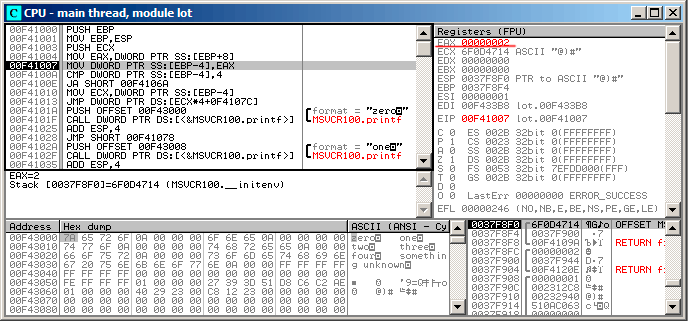
\includegraphics[scale=\FigScale]{patterns/08_switch/2_lot/lot_olly1.png}
\caption{\olly: \RU{входное значение ф-ции загружено в}\EN{function's input value is loaded in} \EAX}
\label{fig:switch_lot_olly1}
\end{figure}

\begin{figure}[H]
\centering
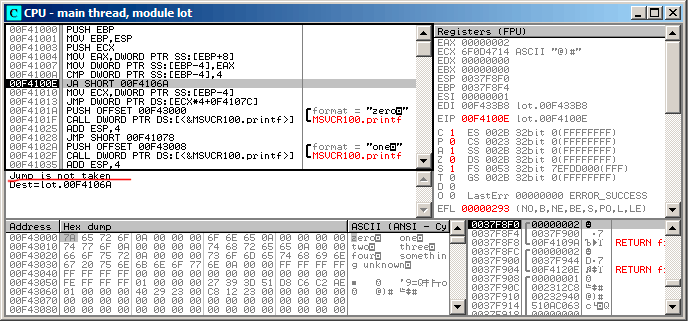
\includegraphics[scale=\FigScale]{patterns/08_switch/2_lot/lot_olly2.png}
\caption{\olly: $2$ \RU{не больше чем}\EN{is no bigger than} $4$: \RU{переход не сработает}\EN{no jump is taken}}
\label{fig:switch_lot_olly2}
\end{figure}

\begin{figure}[H]
\centering
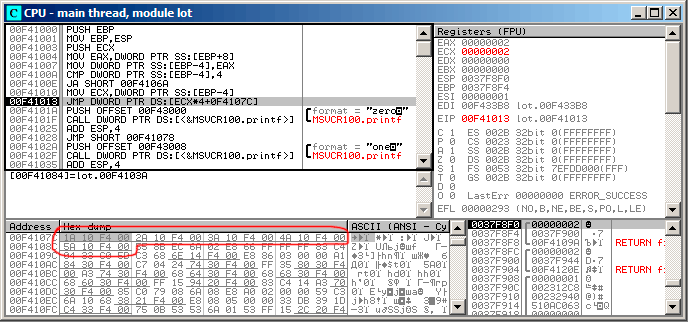
\includegraphics[scale=\FigScale]{patterns/08_switch/2_lot/lot_olly3.png}
\caption{\olly: \RU{вычисляем адрес для перехода используя}\EN{calculating destination address using} jumptable}
\label{fig:switch_lot_olly3}
\end{figure}

\begin{figure}[H]
\centering
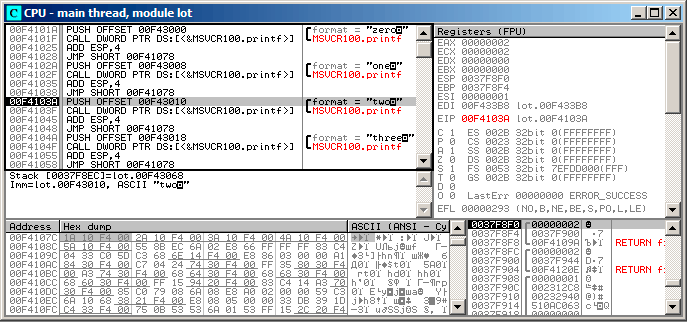
\includegraphics[scale=\FigScale]{patterns/08_switch/2_lot/lot_olly4.png}
\caption{\olly: \RU{теперь мы на соответствующей метке}\EN{now we at corresponding} \IT{case:}\EN{ label}}
\label{fig:switch_lot_olly4}
\end{figure}
\fi

\subsubsection{\NonOptimizing GCC}
\label{switch_lot_GCC}

\RU{Посмотрим, что сгенерирует GCC 4.4.1}\EN{Let's see what GCC 4.4.1 generates}:

\lstinputlisting[caption=GCC 4.4.1]{patterns/08_switch/2_lot/lot_gcc.asm}

\index{x86!\Registers!JMP}
\RU{Практически то же самое, за исключением мелкого нюанса: аргумент из \TT{arg\_0} умножается на 4 
при помощи сдвига влево на 2 бита (это почти то же самое что и умножение на 4)~(\ref{SHR}).
Затем адрес метки внутри функции берется из массива \TT{off\_804855C} и адресуется при помощи 
вычисленного индекса.}
\EN{It is almost the same, except little nuance: argument \TT{arg\_0} is multiplied by 4 by
shifting it to left by 2 bits (it is almost the same as multiplication by 4)~(\ref{SHR}).
Then label address is taken from \TT{off\_804855C} array, address is calculated and stored into 
\EAX, then \TT{``JMP EAX''} do actual jump.}


\ifdefined\IncludeARM
\subsection{ARM: \OptimizingKeilVI (\ARMMode)}
\label{sec:SwitchARMLot}

\lstinputlisting[caption=\OptimizingKeilVI (\ARMMode)]{patterns/08_switch/2_lot/lot_ARM_ARM_O3.asm}

\RU{В этом коде используется та особенность режима ARM, 
что все инструкции в этом режиме имеют фиксированную длину 4 байта.}
\EN{This code makes use of the ARM mode feature in which all instructions have a fixed size of 4 bytes.}

\RU{Итак, не будем забывать, что максимальное значение для $a$ это $4$, всё что выше, должно вызвать
вывод строки}
\EN{Let's keep in mind that the maximum value for $a$ is $4$ and any greater value will cause}
\IT{<<something unknown\textbackslash{}n>>}
\RU{.}\EN{to string printing.}

\index{ARM!\Instructions!CMP}
\index{ARM!\Instructions!ADDCC}
\RU{Самая первая инструкция}\EN{The first} \TT{``CMP R0, \#5''} 
\RU{сравнивает входное значение в $a$ c $5$.}
\EN{instruction compares the input value of $a$ with $5$.}

\RU{Следующая инструкция}\EN{The next} \TT{``ADDCC PC, PC, R0,LSL\#2''}
\footnote{ADD\EMDASH\RU{складывание чисел}\EN{addition}}
\RU{сработает только в случае если}\EN{instruction will execute only if} $R0 < 5$ (\IT{CC=Carry clear / Less than}). 
\RU{Следовательно, если}\EN{Consequently, if} \TT{ADDCC} \RU{не сработает}\EN{does not trigger} 
(\RU{это случай с}\EN{it is a} $R0 \geq 5$\EN{ case}), 
\RU{выполнится переход на метку}\EN{a jump to} 
\IT{default\_case}\RU{.}\EN{ label will occur.}

\RU{Но если}\EN{But if} $R0 < 5$ \AndENRU \TT{ADDCC} \RU{сработает, то произойдет следующее:}
\EN{triggers, the following will happen:}

\RU{Значение в \Reg{0} умножается на $4$}\EN{The value in \Reg{0} will be multiplied by $4$}.
\RU{Фактически}\EN{In fact}, \TT{LSL\#2} \RU{в суффиксе инструкции означает ``сдвиг влево на 2 бита''.}
\EN{at the instruction's suffix means ``shift left by 2 bits''.}
\RU{Но как будет видно позже}\EN{But as we will see later}~(\myref{division_by_shifting}) \RU{в секции}\EN{in section} 
``\ShiftsSectionName'', 
\RU{сдвиг влево на 2 бита это как раз эквивалентно его умножению на $4$.}
\EN{shift left by 2 bits is equivalent to multiplying by $4$.}

\RU{Затем полученное}\EN{Then we add} $R0*4$ \RU{прибавляется к текущему значению \ac{PC}}\EN{to
the current value in \ac{PC}}, 
\RU{совершая, таким образом, переход на одну из расположенных ниже инструкций \TT{B} (\IT{Branch}).}
\EN{thus jumping to one of the \TT{B} (\IT{Branch}) instructions located below.}

\RU{На момент исполнения}\EN{At the moment of the execution of} \TT{ADDCC},
\RU{содержимое \ac{PC} на 8 байт больше}\EN{the value in \ac{PC} is 8 bytes ahead} (\TT{0x180}) 
\RU{чем адрес по которому расположена сама инструкция} 
\EN{than the address at which the} \TT{ADDCC}\EN{ instruction is located} (\TT{0x178}), 
\RU{либо, говоря иным языком, на 2 инструкции больше.}
\EN{or, in other words, 2 instructions ahead.}

\index{ARM!\RU{Конвейер}\EN{Pipeline}}
\RU{Это связано с работой конвейера процессора ARM:
пока исполняется инструкция \TT{ADDCC}, процессор уже начинает обрабатывать инструкцию после следующей, 
поэтому \ac{PC} указывает туда. Этот факт нужно запомнить.}
\EN{This is how the pipeline in ARM processors works: when \TT{ADDCC} is executed,
the processor at the moment
is beginning to process the instruction after the next one,
so that is why \ac{PC} points there. This should be memorized.}

\RU{В случае, если $a=0$, тогда к \ac{PC} ничего не будет прибавлено, 
в \ac{PC} запишется актуальный на тот момент \ac{PC} (который больше на 8) 
и произойдет переход на метку \IT{loc\_180}, 
это на 8 байт дальше от места где находится инструкция \TT{ADDCC}.}
\EN{If $a=0$, then nothing will be added to the value in \ac{PC},
and the actual value in the \ac{PC} will be written into \ac{PC} (which is 8 bytes ahead)
and a jump to the label \IT{loc\_180} will happen,
which is 8 bytes ahead of the point where the \TT{ADDCC} instruction is.}

\RU{В случае, если}\EN{If} $a=1$, \RU{тогда в \ac{PC} запишется}\EN{then} 
$PC+8+a*4 = PC+8+1*4 = PC+12 = 0x184$\RU{, это адрес метки \IT{loc\_184}}\EN{ will be written to \ac{PC},
which is the address of the \IT{loc\_184} label}.

\RU{При каждой добавленной к $a$ единице, итоговый \ac{PC} увеличивается на $4$.}
\EN{With every $1$ added to $a$, the resulting \ac{PC} is increased by $4$.}
\RU{$4$ это как раз длина инструкции  в режиме ARM и одновременно с этим, 
длина каждой инструкции \TT{B}, их здесь следует 5 в ряд.}
\EN{$4$ is the instruction length in ARM mode and also, the length of each \TT{B} instruction,
of which there are 5 in row.}

\RU{Каждая из этих пяти инструкций \TT{B}, передает управление дальше, где собственно и происходит то, 
что запрограммировано в}
\EN{Each of these five \TT{B} instructions passes control further, to 
what was programmed in the}
\IT{switch()}.
\RU{Там происходит загрузка указателя на свою строку, и т.д.}
\EN{Pointer loading of the corresponding string occurs there, etc.}

\subsection{ARM: \OptimizingKeilVI (\ThumbMode)}

\lstinputlisting[caption=\OptimizingKeilVI (\ThumbMode)]{patterns/08_switch/2_lot/lot_ARM_thumb_O3.asm}

\index{ARM!\ThumbMode}
\index{ARM!\ThumbTwoMode}
\RU{В режимах thumb и thumb-2, уже нельзя надеяться на то что все инструкции будут иметь одну длину.}
\EN{One cannot be sure that all instructions in thumb and thumb-2 modes will have the same size.}
\RU{Можно даже сказать, что в этих режимах инструкции переменной длины, как в x86.}
\EN{It can even be said that in these modes the instructions have variable lengths, just like in x86.}

\index{jumptable}
\RU{Так что здесь добавляется специальная таблица, содержащая информацию о том, как много вариантов здесь,
не включая default-варианта, и смещения, для каждого варианта, каждое кодирует метку, куда нужно передать
управление в соответствующем случае.}
\EN{So there is a special table added that contains information about how much cases are there (not including 
default-case), and an offset for each with a label to which control must be passed in 
the corresponding case.}

\index{ARM!\RU{Переключение режимов}\EN{Mode switching}}
\index{ARM!\Instructions!BX}
\RU{Для того чтобы работать с таблицей и совершить переход, вызывается служебная функция}
\EN{A special function is present here in order to deal with the table and pass control, named} \\
\IT{\_\_ARM\_common\_switch8\_thumb}. 
\RU{Она начинается с инструкции}\EN{It starts with} \TT{``BX PC''}
\RU{, чья функция ~--- переключить процессор в ARM-режим.}
\EN{, whose function is to switch the processor to ARM-mode.}
\RU{Далее функция, работающая с таблицей.}\EN{Then you see the function for table processing.} 
\RU{Она слишком сложная для 
рассмотрения в данном месте, так что я пропущу все объяснения.}
\EN{It is too complex to describe it here now, so I will omit it.}
% TODO дописать когда-то?

\index{ARM!\Registers!Link Register}
\RU{Но можно отметить, что эта функция использует регистр \ac{LR} как указатель на таблицу.}
\EN{It is interesting to note that the function uses the \ac{LR} register as a pointer to the table.}
\RU{Действительно, после вызова этой функции, в \ac{LR} был записан
адрес после инструкции}\EN{Indeed, after this calling this function, \ac{LR} will contain the address after} \\ 
\TT{``BL \_\_ARM\_common\_switch8\_thumb''}\RU{, а там как раз и начинается таблица.}
\EN{ instruction, where the table starts.}

\RU{Еще можно отметить что код для этого выделен в отдельную функцию для того, 
чтобы не нужно было каждый раз генерировать 
точно такой же фрагмент кода для каждого выражения switch().}
\EN{It is also worth noting that the code is generated as a separate function in order to reuse it, 
so the compiler will not generate the same code for every switch() statement.}

\IDA 
\RU{распознала эту служебную функцию и таблицу автоматически, дописав комментарии к меткам вроде}
\EN{successfully perceived it as a service function and a table, and added comments to the labels
like}\\
\TT{jumptable 000000FA case 0}.


\fi
\ifdefined\IncludeMIPS
\subsection{MIPS}

\lstinputlisting[caption=\Optimizing GCC 4.4.5 (IDA)]{patterns/08_switch/2_lot/MIPS_O3_IDA.lst.\LANG}

\index{MIPS!\Instructions!SLTIU}
\RU{Новая для нас инструкция здесь это SLTIU (``Set on Less Than Immediate Unsigned''~--- установить,
если меньше чем значение, беззнаковое сравнение).}
\EN{The new instruction for us is SLTIU (``Set on Less Than Immediate Unsigned'').}
\index{MIPS!\Instructions!SLTU}
\RU{На самом деле, это то же что и SLTU (``Set on Less Than Unsigned''), но ``I'' означает ``immediate'',
т.е. число может быть задано в самой инструкции.}
\EN{This is the same as SLTU (``Set on Less Than Unsigned''), but ``I'' stands for ``immediate'', 
i.e., a number has to be specified in the instruction itself.}

\index{MIPS!\Instructions!BNEZ}
BNEZ \RU{это}\EN{is} ``Branch if Not Equal to Zero''\RU{ (переход если не равно нулю)}.

\RU{Код очень похож на код для других \ac{ISA}.}\EN{Code is very close to the other \ac{ISA}s.}
\index{MIPS!\Instructions!SLL}
SLL (``Shift Word Left Logical''\RU{~--- логический сдвиг влево}) 
\RU{совершает умножение на 4}\EN{does multiplication by 4}.
\RU{MIPS всё-таки это 32-битный процессор, так что все адреса в таблице переходов 
(\IT{jumptable}) 32-битные.}
\EN{MIPS is a 32-bit CPU after all, so all addresses in the \IT{jumptable} are 32-bit ones.}

\fi

\subsection{\Conclusion{}}

\RU{Примерный скелет}\EN{Rough skeleton of} \IT{switch()}:

% TODO:  ARM, MIPS skeleton
\lstinputlisting[caption=x86]{patterns/08_switch/2_lot/skel1.lst.\LANG}

\RU{Переход по адресу из таблицы переходов может быть также реализован такой инструкцией:}
\EN{The jump to the address in the jump table may also be implemented using this instruction:}
\TT{JMP jump\_table[REG*4]}.
\RU{Или}\EN{Or} \TT{JMP jump\_table[REG*8]} \InENRU x64.

\RU{Таблица переходов (\IT{jumptable}) это просто массив указателей, как это будет вскоре описано:}
\EN{A \IT{jumptable} is just array of pointers, like the one described later:}
\ref{array_of_pointers_to_strings}.

% TODO What's the difference between 3 and 4? Seems to be the same...
% it is fallthrough from 3 to 4 :) --DY
\section{\RU{Когда много \IT{case} в одном блоке}
\EN{When there are several \IT{case} in one block}}

\RU{Вот очень часто используемая конструкция: несколько \IT{case} может быть использовано в одном блоке:}
\EN{Here is also a very often used construction: several \IT{case} statements may be used in single block:}

\lstinputlisting{patterns/08_switch/3_several_cases/several_cases.c}

\RU{Слишком расточительно генерировать каждый блок для каждого случая, поэтому обычно
каждый блок генерируется плюс диспетчер.}
\EN{It's too wasteful to generate each block for each possible case,
so what is usually done, is each block generated plus some kind of dispatcher.}

\subsection{MSVC}

\lstinputlisting[caption=\Optimizing MSVC 2010,numbers=left]{patterns/08_switch/3_several_cases/several_cases_MSVC_2010_Ox.asm.\LANG}

\RU{Здесь видим две таблицы}\EN{We see two tables here}: 
\RU{первая таблица}\EN{the first table} (\TT{\$LN10@f}) \RU{это таблица индексов}\EN{is index table},
\RU{и вторая таблица}\EN{and the second table} (\TT{\$LN11@f}) \RU{это массив указателей на блоки}\EN{is 
an array of pointers to blocks}.

\RU{В начале, входное значение используется как индекс в таблице индексов}\EN{First, input value 
is used as index in index table} (\LineENRU 13). 

\RU{Вот краткое описание значений в таблице}\EN{Here is short legend for values in the table}: 
0 \RU{это первый блок \IT{case}}\EN{is first \IT{case} block} (\RU{для значений}\EN{for values} 1, 2, 7, 10),
1 \RU{это второй}\EN{is second} (\RU{для значений}\EN{for values} 3, 4, 5),
2 \RU{это третий}\EN{is third} (\RU{для значений}\EN{for values} 8, 9, 21),
3 \RU{это четвертый}\EN{is fourth} (\RU{для значений}\EN{for value} 22),
4 \RU{это для default-блока}\EN{is for default block}.

\RU{Мы получаем индекс для второй таблицы указателей на блоки и переходим туда}\EN{We get there index for 
the second table of block pointers and we jump there} (\LineENRU 14).

\EN{What is also worth to note that there are no case for input value $0$.}
\RU{Что еще нужно отметить, так это то что здесь нет случая для нулевого входного значения.}
\EN{Hence, we see \DEC instruction at line 10, and the table is beginning at $a=1$. 
Because there are no need to allocate table element for $a=0$.}
\RU{Поэтому мы видим инструкцию \DEC на строке 10 и таблица начинается с $a=1$.
Потому что незачем выделять в таблице элемент для $a=0$.}

\RU{Это очень часто используемый шаблон}\EN{This is very often used pattern}.

\RU{В чем же экономия}\EN{So where economy is}?
\RU{Почему нельзя сделать так, как уже обсуждалось}\EN{Why it's not possible to make it as it was 
already discussed} (\ref{switch_lot_GCC}), \RU{используя только одну таблицу, содержащую указатели на 
блоки}\EN{just with one table, consisting of block pointers}?
\RU{Причина в том, что элементы в таблице индексов занимают только по 8-битному байту, поэтому всё это более 
компактно}\EN{The reason is that elements in index table has 8-bit byte type, hence it's all more compact}.

\subsection{GCC}

GCC \RU{делает так, как уже обсуждалось}\EN{do the job like it was already discussed} 
(\ref{switch_lot_GCC}), \RU{используя просто таблицу указателей}\EN{using just one table of pointers}.

\subsection{ARM64: \Optimizing GCC 4.9.1}

\RU{Во-первых, здесь нет кода, срабатывающего в случае если входное значение --- 0, так что GCC пытается
сделать таблицу переходов более компактной и начинает с случая, когда входное значение --- 1.}
\EN{First of all, there are no code triggering if input value is 0, so GCC tries to make jumptable more compact
and so it's started at the case of 1 as input value.}

GCC 4.9.1 \ForENRU ARM64 \RU{использует даже более интересный трюк}\EN{uses even cleverer trick}.
\RU{Он может закодировать все смещения как 8-битные байты}\EN{It's able to encode all offsets as 8-bit bytes}.
\RU{Вспомним что все инструкции в ARM64 имеют размер в 4 байта.}
\EN{Let's remind ourselves, all ARM64 instructions has size of 4 bytes.}
\RU{GCC также использует тот факт, что все смещения в моем крохотном примере находятся достаточно близко 
друг от друга.}
\EN{GCC is also use the fact that all offsets in my tiny example are in close proximity to each other.}
\RU{Так что таблица переходов состоит из байт.}\EN{So the jumptable consisting of bytes.}

\lstinputlisting[caption=\Optimizing GCC 4.9.1 ARM64]{patterns/08_switch/3_several_cases/ARM64_GCC491_O3.s.\LANG}

\RU{Я скомпилировал мой пример как объектный файл и открыл его в IDA. Вот таблица переходов:}
\EN{I just compiled my example to object file and opened it in IDA. Here is a jump table:}

\lstinputlisting[caption=jumptable in IDA]{patterns/08_switch/3_several_cases/ARM64_GCC491_O3_IDA.lst}

\RU{В случае 1, 9 будет умножено на 9 и прибавлено к адресу метки Lrtx4.}
\EN{So in case of 1, 9 will be multiplied by 4 and added to the address of Lrtx4 label.}
\RU{В случае 22, 0 будет умножено на 4, в результате это 0.}
\EN{In case of 22, 0 is to be multiplied by 4 resulting 0. }
\RU{Место сразу за меткой Lrtx4, это метка L7, где находится код выводящий ``22''.}
\EN{The place right after Lrtx4 label is L7 label, where the code printing ``22'' is.}
\RU{В сегменте кода нет таблицы переходов, место для нее выделено в отдельной секции .rodata
(нет особой нужды располагать её в сегменте кода).}
\EN{There are no jumptable in the code segment, a place for it is allocated in separate .rodata section 
(there are no special need to place it in code section).}

\RU{Там есть также отрицательные байты (0xF7), они используются для перехода назад, на код выводящий
строку ``default'' (на .L2).}
\EN{There are also negative bytes (0xF7), they are used for jumping back to the code printing ``default'' string 
(at .L2).}

\section{Fall-through}

\RU{Еще одно популярное использование}\EN{Another very popular usage of} \TT{switch()} 
\EN{is the fall-through}\RU{это т.н. ``fallthrough'' (``проваливаясь'')}.
\RU{Вот простой пример}\EN{Here is a small example}:

\lstinputlisting[numbers=left]{patterns/08_switch/4_fallthrough/fallthrough.c}

\RU{Если}\EN{If} $type=1$ (R), $read$ \RU{будет выставлен в}\EN{will be set to} $1$, \RU{если}\EN{if} 
$type=2$ (W), $write$ \RU{будет выставлен в}\EN{will be set to} $2$.
\RU{В случае}\EN{In case of} $type=3$ (RW), \RU{обе}\EN{both} $read$ \AndENRU $write$ \RU{будут 
выставлены в}\EN{will be set to} $1$.

\RU{Фрагмент кода на строке 14 будет исполнен в двух случаях: если}\EN{The code at 
line 14 is executed in two cases: if} $type=RW$ \RU{или если}\EN{or if} $type=W$.
\RU{Там нет ``break'' для ``case RW'', и это нормально}\EN{There is no ``break'' 
for ``case RW''x and that's OK}.

\subsection{MSVC x86}

\lstinputlisting[caption=MSVC 2012]{patterns/08_switch/4_fallthrough/fallthrough_MSVC.asm}

\RU{Код почти полностью повторяет то что в исходнике.}
\EN{The code mostly resembles what is in the source.}
\RU{Там нет переходов между метками}\EN{There are no jumps between labels} \TT{\$LN4@f} \AndENRU 
\TT{\$LN3@f}: \RU{так что когда управление (code flow) находится на}\EN{so when code flow is at} 
\TT{\$LN4@f}, $read$ \RU{в начале выставляется в $1$, затем}\EN{is first set to $1$, then} $write$.
\EN{This is why it's called fall-through: code flow falls through one piece of code
(setting $read$) to another (setting $write$).}
\RU{Наверное, поэтому всё это и называется ``проваливаться'': управление проваливается через
один фрагмент кода (выставляющий $read$) в другой (выставляющий $write$).}
\RU{Если}\EN{If} $type=W$, \RU{мы оказываемся на}\EN{we land at} \TT{\$LN3@f}, 
\RU{так что код выставляющий $read$ в $1$ не исполнится}\EN{so no code setting $read$ to $1$ 
is executed}.

\ifdefined\IncludeARM
\subsection{ARM64}

\lstinputlisting[caption=GCC (Linaro) 4.9]{patterns/08_switch/4_fallthrough/fallthrough_ARM64.s.\LANG}

\RU{Почти то же самое}\EN{Merely the same thing}.
\RU{Здесь нет переходов между метками}\EN{There are no jumps between labels} \TT{.L4} 
\AndENRU \TT{.L3}.
\fi


\ifdefined\IncludeExercises
\section{\Exercises}

\subsection{\Exercise \#1}
\label{exercise_switch_1}

\RU{Вполне возможно переделать пример на Си в листинге \myref{switch_lot_c} так, чтобы при компиляции
получалось даже ещё меньше кода, но работать всё будет точно так же.}
\EN{It's possible to rework the C example in \myref{switch_lot_c} in such way that the compiler
can produce even smaller code, but will work just the same.}
\RU{Попробуйте этого добиться}\EN{Try to achieve it}.

\RU{Подсказка}\EN{Hint}: \myref{exercise_solutions_switch_1}.
\fi
